\section{Clustering analysis}
\subsection{Preprocessing}
In order to let the cluster algorithms work, we had to preprocess the data. Initially we tried to use the MinMax scaler, but we saw that K-Means was not working well. Due to that, we decided to normalize such features with their z-score by using the scikit-learn StandardScaler method. 

\subsection{K-Means}
\subsubsection{Feature selection} In order to apply K-Means, we selected only some  features to avoid the course of dimensionality. \textbf{We selected the attributes that best differentiate strong players from weak ones}. We have also tried the PCA (principal components' analysis) approach to understand the most relevant features, but the results, obtained by the K-Means on these features, were not satisfying in terms of silhouette score. After several experiments, we obtained the best result choosing as parameters the number of tourney won (\textit{t\_won}), the percentage of wins (\textit{p\_wins}) and the rank (\textit{rank}) of each player.
We also tried different set of features (percentage of wins on each surface and statics) which we also explored with the k-means algorithm, but the explanation of the results it's not easy for someone who isn't fond of tennis, so we decided to work mainly with the three features listed before.

\subsubsection{Choosing the best K}
The choice of the parameter k in the k-means approach is crucial since it identifies the number of clusters resulting from the algorithm's execution, but before choosing the best k we let the algorithm work for twenty times and then we analyzed the indicators in \autoref{fig:kmeansMetrics}. We choose $k=3$ by following the informal elbow rule for the SSE graph in \autoref{fig:KMeansK}, moreover we wanted an high value for the silhoutte score and a low one for the Davies-Bouldin score as we can see for $k=3$ on \autoref{fig:kmeansMetrics}.
\begin{figure}[H]
    \centering
    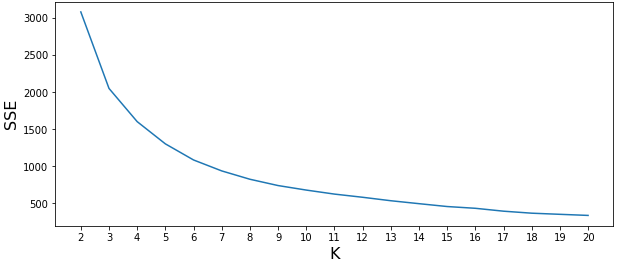
\includegraphics[width=0.45\linewidth]{images/clustering/KMeans/KMeans_K.png}
    \caption{K-Means SSE over K clusters.}
    \label{fig:KMeansK}
\end{figure}
\begin{figure}[H]
    \centering
    \subfloat[K-Means silohuette score]{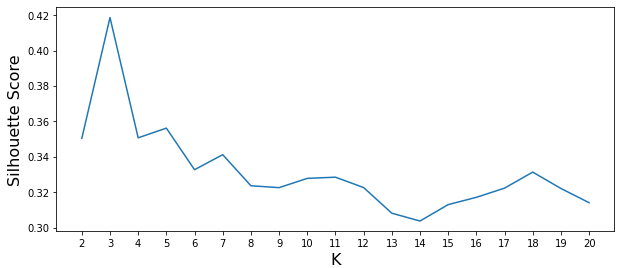
\includegraphics[width=0.45\linewidth]{images/clustering/KMeans/KMeans_Siluette.png}}
    \subfloat[K-Means Davies-Bouldin Score]{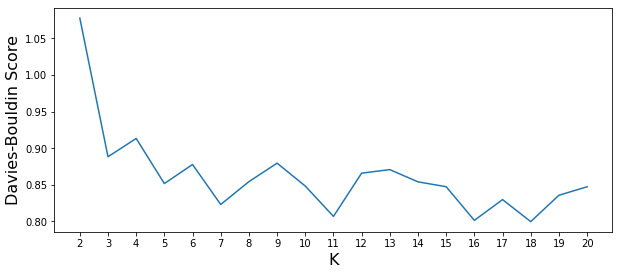
\includegraphics[width=0.45\linewidth]{images/clustering/KMeans/KMeans_Davies.png}}
    \caption{K-Means metrics over k clusters.}
    \label{fig:kmeansMetrics}
\end{figure}

\subsubsection{Cluster analysis}
We applied the PCA on the previously chosen features to analyze the K-means results, then we showed the scatterplot of the first two principal components. As we can see in \autoref{fig:KMeansOut}, the players are divided from left to right by their skills: the weak ones, the average ones and the strong ones. The points on the top right correspond to the top tennis players, such as Djokovic, Nadal and Zverev; we have highlighted Novak Djokovic, the player with rank 1, in the plot to better show the distribution of the players by strength. We have noticed that some players with a high rank are in cluster 0, this is probably due to the fact that they have a high win rate or have won some minor tournaments.

\begin{figure}[H]
    \centering
    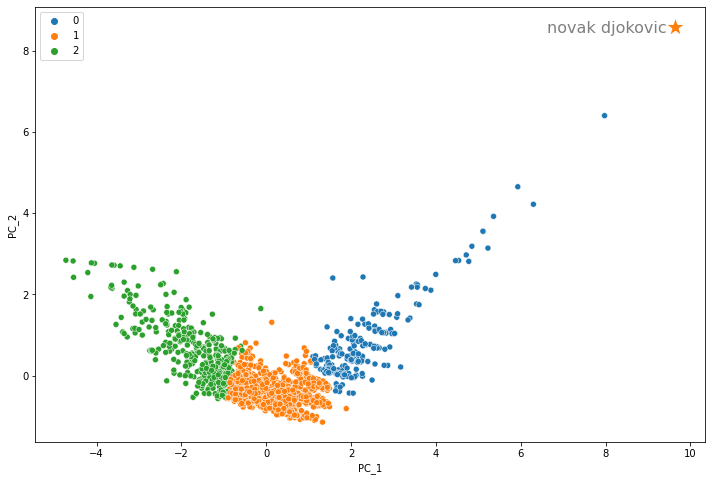
\includegraphics[width=0.5\linewidth]{images/clustering/KMeans/KMeans_out.png}
    \caption{The 3 clusters obtained using K-Means.}
    \label{fig:KMeansOut}
\end{figure}

\begin{figure}[H]
    \centering
    \subfloat{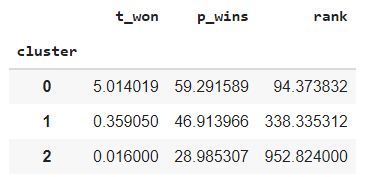
\includegraphics[width=0.30\linewidth]{images/clustering/KMeans/KMeans_stats_avg.png}}
    \subfloat{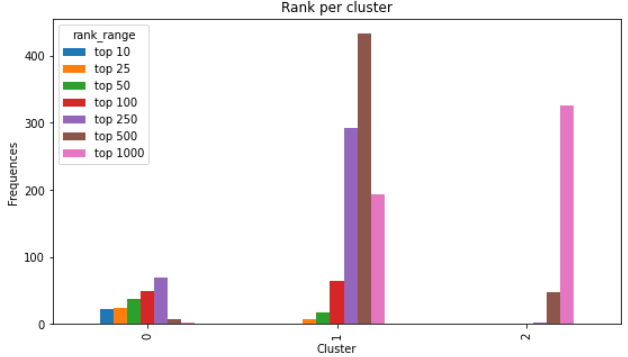
\includegraphics[width=0.3\linewidth]{images/clustering/KMeans/KMeans_stats.png}}
    \caption{Statistics of the feature for each cluster.}
    \label{fig:kmeansAvg}
\end{figure}

\subsection{DBScan}
We decided to work with the dataframe used in the k-means analysis (the one with "t\_won", "p\_wins", "rank"), since we think that it better describes who are the best players and those who aren't.

\subsubsection{Determining eps and min points}
The distance between data points is computed using the Euclidean metric, and for selecting the best eps and min\_samples values we first performed a grid search whose results can be found on the notebook. From the results we choose $min\_samples=8$ and by looking at \autoref{fig:DBScanDist} we choose $eps=0.55$ since it's the value at which the graph's curvature is the highest. The silhouette score is equal to 0.6208

\begin{figure}[H]
    \centering
    \subfloat{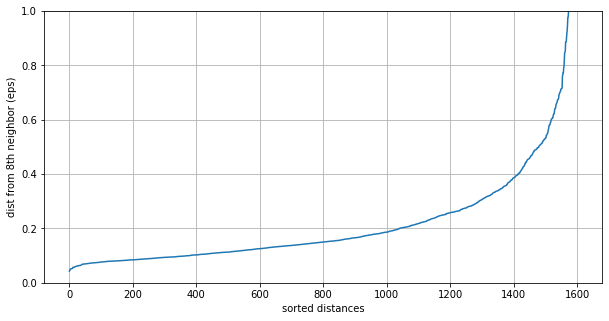
\includegraphics[width=0.45\linewidth]{images/clustering/DBScan/DBScan_dist.png}}
    \subfloat{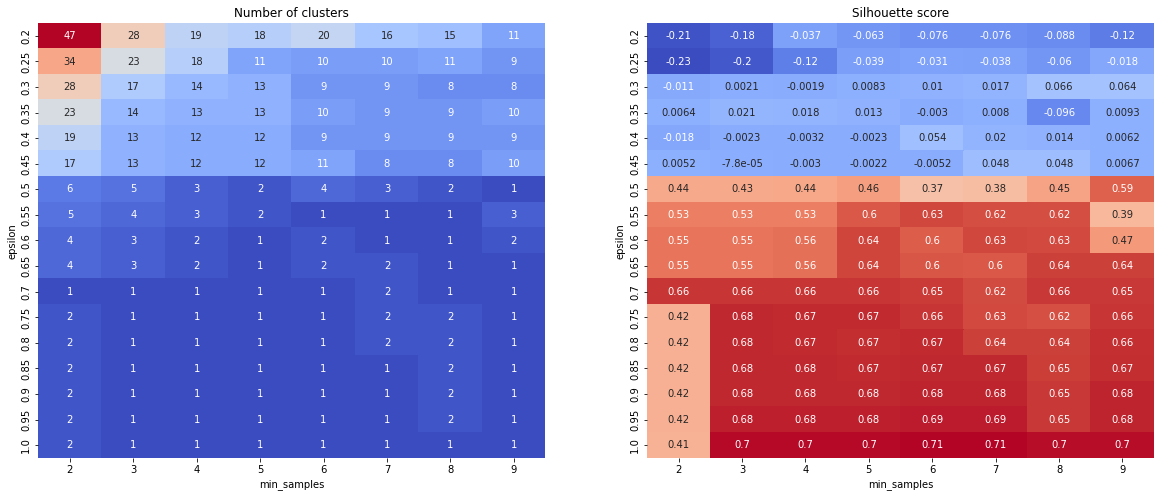
\includegraphics[width=0.55\linewidth]{images/clustering/DBScan/DBScan_grid.png}}
    \caption{DBScan: determining eps and min\_samples}
    \label{fig:DBScanDist}
\end{figure}

\subsubsection{Cluster analysis}
Analyzing the clusters obtained by the DBScan method (\autoref{fig:DBScanOut}), we've seen that there is a single large cluster (the orange one) and the blue points referring to the outliers. In the outliers' cluster there are the players at the extremes: the players who have won very few matches and the strongest players in the world, respectively on the left and right side of the main clsuter. There are also outliers in the center of the plot, representing players who have won some minor tournaments.

\begin{figure}[H]
    \centering
    \subfloat[Clusters generated by applying DBScan, plotted along the 2 P.C.]{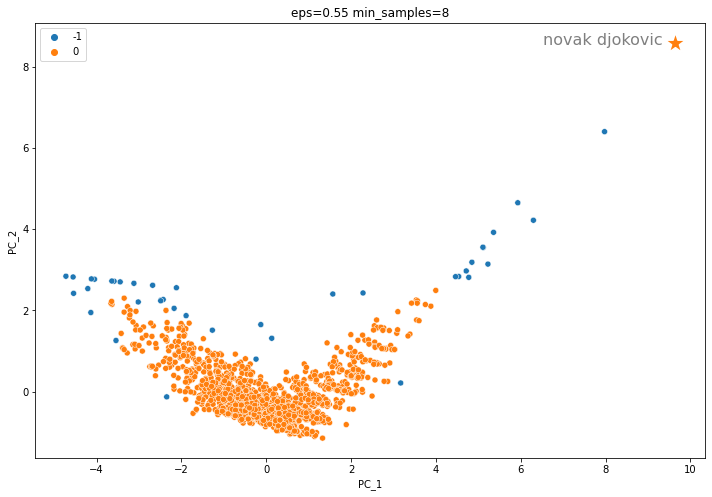
\includegraphics[width=0.52\linewidth]{images/clustering/DBScan/DBScan_out.png}}
    \subfloat[Distribution of players' ranks per cluster]{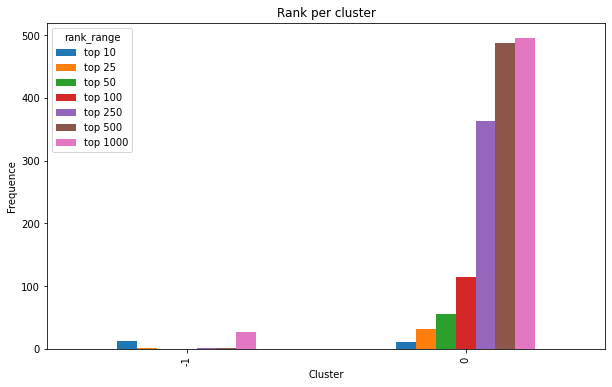
\includegraphics[width=0.48\linewidth]{images/clustering/DBScan/DBScan_rank_clust.png}}
    \caption{DBScan: cluster analysis.}
    \label{fig:DBScanOut}
\end{figure}

\subsection{Hierachical Clustering}
The analysis of the clustering via hierarchical clustering has been conducted using the same set of attributes of the previous algorithms, in order to get results comparable in terms of indicators and properties among the approaches.

\subsubsection{Distance methods}
Like we did with the other clustering algorithms, we used the Euclidean metric to compute the distance between the pairs of points. We have tried several type of agglomerative clustering that differ by the merging criterion of the clusters like min, max, average and ward. In the hierarchical clustering approach, we have not assumed any particular number of clusters: any desired number of clusters can be obtained by ‘cutting’ the dendrogram at the proper level.

\subsubsection{Comparing dendrograms}
\paragraph{Cut threshold} The "best cut" of the dendrograms, is a cut that passes from the longest vertical segment not interrupted by horizontal lines. Anyway we avoided to choose a cut that would have produced too unbalanced clusters.

\begin{table}[H]
\centering
\begin{tabular}{l|l|l}
\textbf{Method}   & \textbf{cluster id : its dimension} & \textbf{Silhouette} \\\hline
Complete & 0: 759, \hspace{2pt} 1: 12, \hspace{2pt} 2: 827, \hspace{2pt} 3: 2 & 0.3082\\
Single   & 0: 1598, 1: 1, \hspace{2pt} \hspace{2pt} 2: 1 & 0.8013 \\
Average  & 0: 1580, 1: 2, \hspace{2pt} \hspace{2pt} 2: 18 & 0.6485 \\
Ward     & 0: 330, \hspace{2pt} 1: 296, 2: 974 & 0.3756 \\\hline  
\end{tabular}
\end{table}
Even if the silhouette is pretty good using the single and average methods, we can not say the same thing looking at the dendrograms, since the clusters are unbalanced, and as a consequence, most of the points falls in one big cluster. The only exceptions in this behaviour is produced by applying Ward method, that produced an almost balanced clusters closer to the K-Means ones, as shown in \autoref{fig:hier_clusters}.

\begin{figure}[H]
    \centering
    \subfloat[Complete]{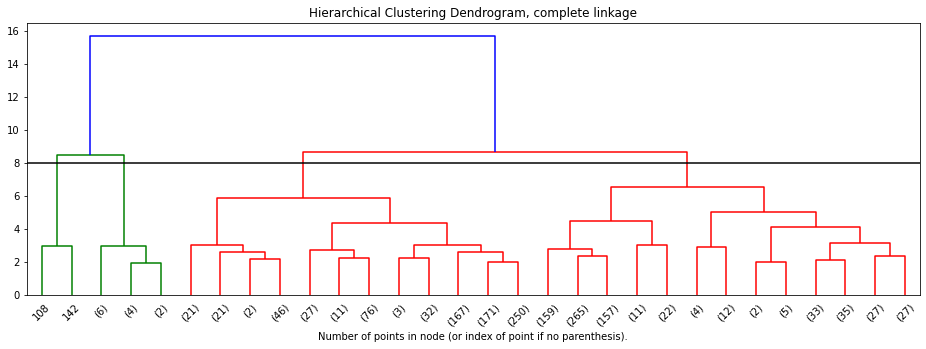
\includegraphics[width=0.5\linewidth]{images/clustering/Hierarchical/Hierac_complete.png}}
    \subfloat[Single]{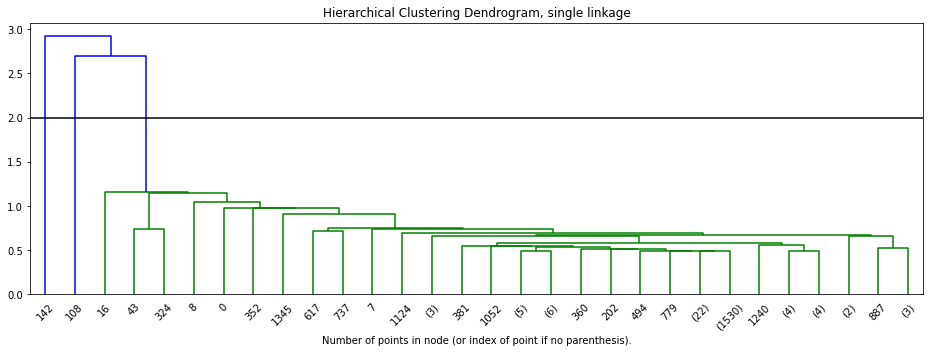
\includegraphics[width=0.5\linewidth]{images/clustering/Hierarchical/Hierac_single.png}}\\
    \subfloat[Average]{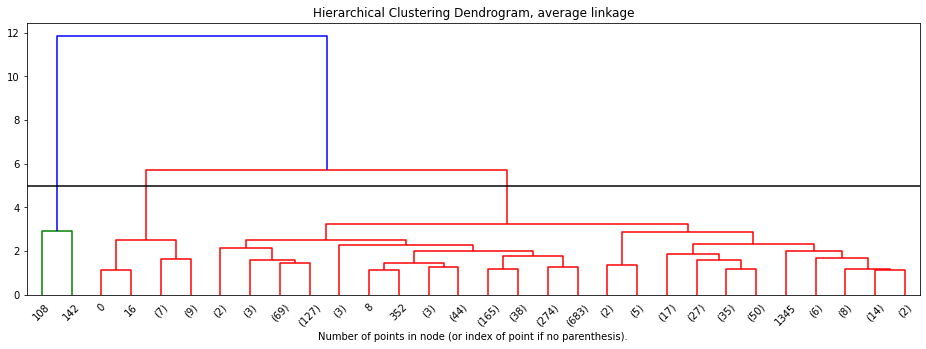
\includegraphics[width=0.5\linewidth]{images/clustering/Hierarchical/Hierac_avg.png}}
    \subfloat[Ward]{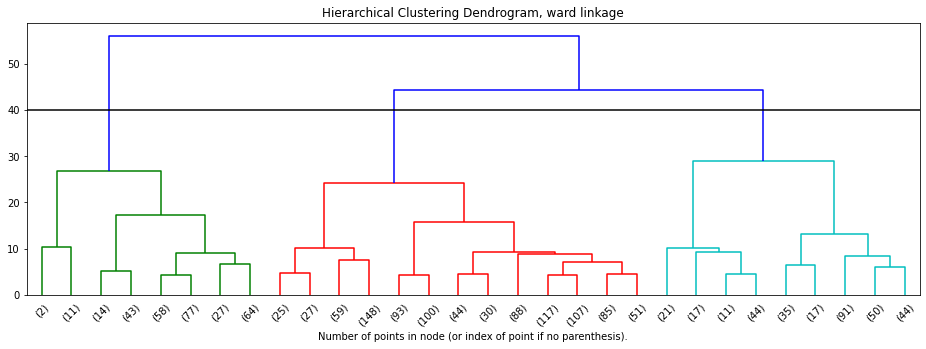
\includegraphics[width=0.5\linewidth]{images/clustering/Hierarchical/Hierac_ward.png}}
    \caption{Hierarchical clustering methods comparison: dendrograms.}
    \label{fig:hier_dendograms}
\end{figure}

\subsubsection{Comparing clusters}
By looking at the pcas plot from \autoref{fig:hier_clusters}, we can define the hierarchical clusterings with complete and ward linkage as the best ones among the four methods. The single linkage was the worst one since it created two cluster with one player each (Djokivic and Nadal which are the best overall player), meanwhile the average one separated the extremely strong players (again Djokivic and Nadal) from the strong ones (green cluster) and the average or weak ones (blue cluster). The only approach that didn't have such drastic separation were the complete and ward linkages, which is why we considered them as the best among foru approaches.
\begin{figure}[H]
    \centering
    \subfloat[Complete]{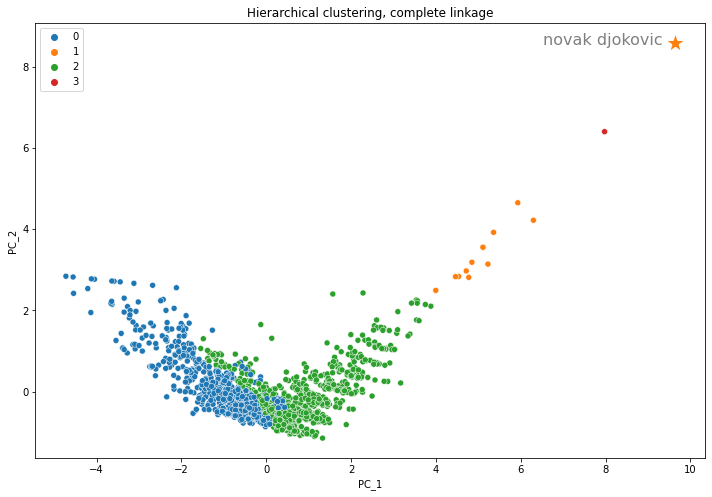
\includegraphics[width=0.4\linewidth]{images/clustering/Hierarchical/Hierac_complete_cluster.png}}
    \subfloat[Single]{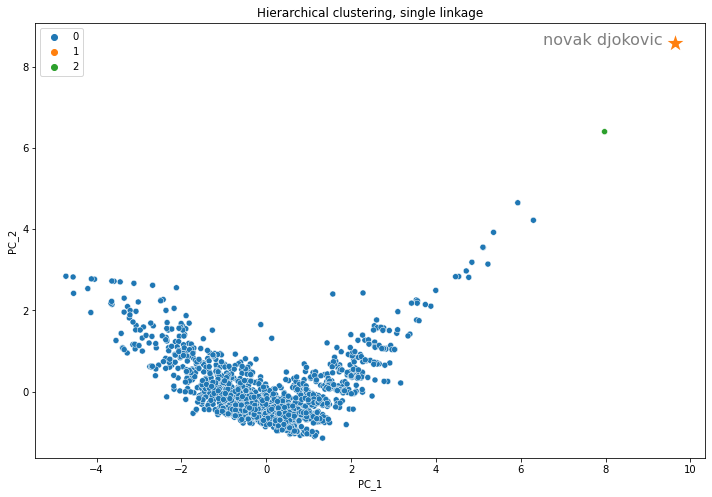
\includegraphics[width=0.4\linewidth]{images/clustering/Hierarchical/Hierac_single_cluster.png}}\\
    \subfloat[Average]{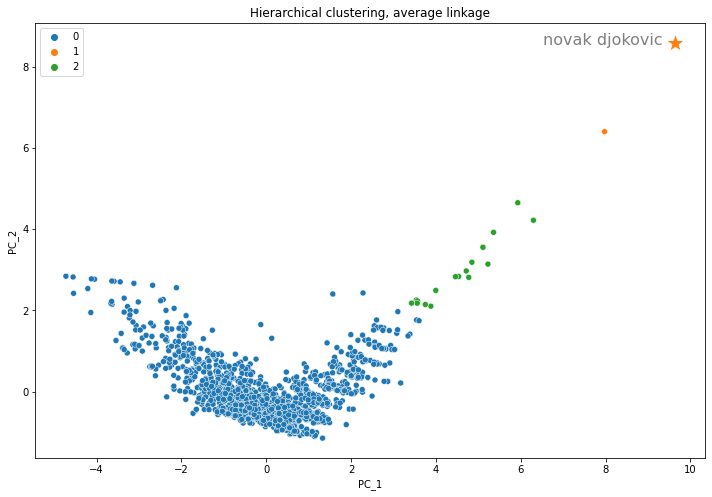
\includegraphics[width=0.4\linewidth]{images/clustering/Hierarchical/Hierac_avg_cluster.png}}
    \subfloat[Ward]{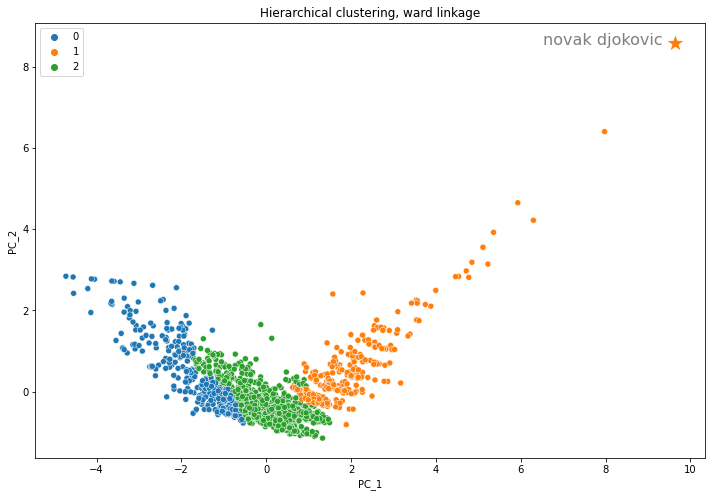
\includegraphics[width=0.4\linewidth]{images/clustering/Hierarchical/Hierac_ward_cluster.png}}
    \caption{Hierarchical clustering: plotting along the PCAs.}
    \label{fig:hier_clusters}
\end{figure}

\subsection{Validation by external measures}
We computed the \textit{similarity matrix} $S$ given a particular clustering. To obtain this matrix, the indices are sorted according to the labels of the clusters and the component $S(i,j)$ is equal to $e^{-d(i,j)}$, where $d(i,j)$ is the euclidean distance between the points $i$ and $j$. If we have well-separated clusters, then the similarity matrix should be roughly block-diagonal. We also computed the entropy of each feature per cluster: a low entropy score of each attribute indicates a more predictable and less uncertain trend within the clusters. 

\begin{figure}[H]
    \centering
    \subfloat[Similarity Kmeans]{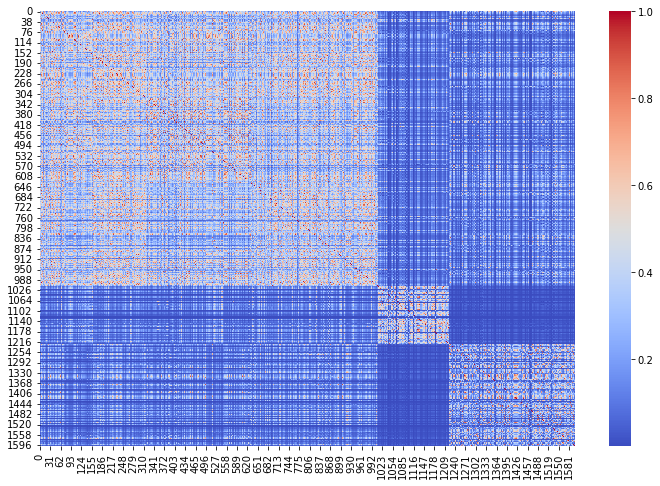
\includegraphics[width=0.3\linewidth]{images/clustering/Validation/KmeansSimMatrix.png}}
    \subfloat[Entropy Kmeans]{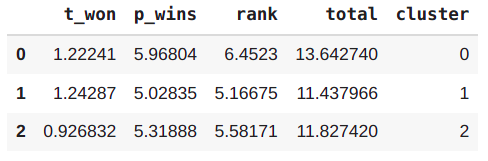
\includegraphics[width=0.3\linewidth]{images/clustering/Validation/kmeansEntropy.png}}\\
    \subfloat[Similarity\\Complete]{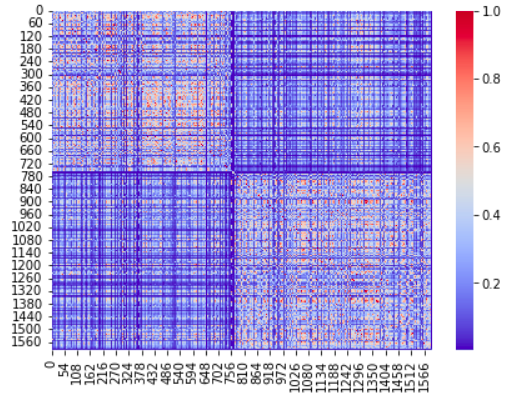
\includegraphics[width=0.3\linewidth]{images/clustering/Validation/completeSimMatrix.png}}   
    \subfloat[Entropy Complete]{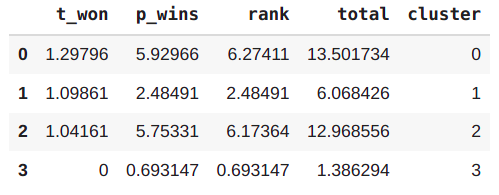
\includegraphics[width=0.3\linewidth]{images/clustering/Validation/completeEntropy.png}}\\
    \subfloat[Similarity\\Ward]{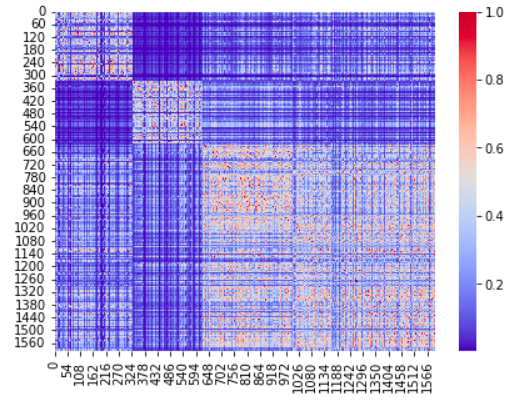
\includegraphics[width=0.3\linewidth]{images/clustering/Validation/SimWard.png}}   
    \subfloat[Entropy Ward]{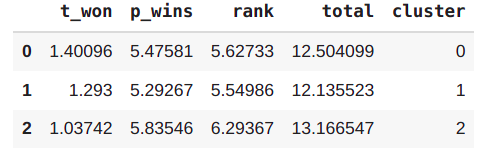
\includegraphics[width=0.3\linewidth]{images/clustering/Validation/EntropyWard.png}}\\
    \subfloat[Entropy Single]{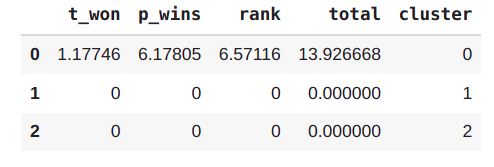
\includegraphics[width=0.3\linewidth]{images/clustering/Validation/EntropySingle.png}}
    \subfloat[Entropy Average]{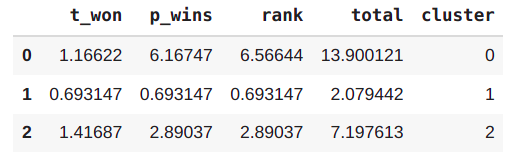
\includegraphics[width=0.3\linewidth]{images/clustering/Validation/EntropyAv.png}}
    \caption{Similarity matrices and Entropy of attributes per cluster for each method}
    \label{fig:val_clusters}
\end{figure}

\iffalse
We compute the \textit{cross-correlation} between the \textit{similarity matrix} of the clustering and the \textit{incidence matrix} (where the component $(i, j)$ is equal to $1$ if $i$ and $j$ are in the same cluster, $0$ otherwise). The \textit{incidence matrix} represents the similarity matrix of a perfect clustering, so high-values component of the cross-correlation matrix represents an high correlation of the two matrix in that offset.
\fi

\subsection{Other Clustering approaches explored}
For the final work on clustering we went to explore two more approaches from the pyclustering package as suggested by the professor, our choice fell on X-Means and SOM soft-clustering.
\subsubsection{X-Means}
From the pyclustering package documentation: X-means clustering method starts with the assumption of having a minimum number of clusters, and then dynamically increases them. X-means uses specified splitting criterion to control the process of splitting clusters.
\vspace{3mm}

This approach is different from the previous ones we tried, since it doesn't need to know beforehand the number of clusters, but it starts with a pre-determined amount and then splits them into smaller ones. The results change from one try to another, but we've seen that this approach usually worked better for our dataframe.
\begin{figure}[H]
    \centering
    \subfloat[Clusters generated by X-Means]{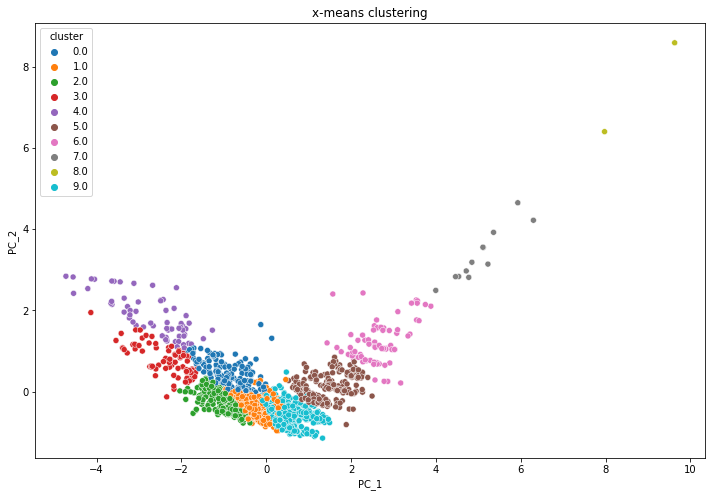
\includegraphics[width=0.38\linewidth]{images/clustering/OtherClusterings/x_means_pca.png}}
    \subfloat[Distribution of players' ranks per cluster]{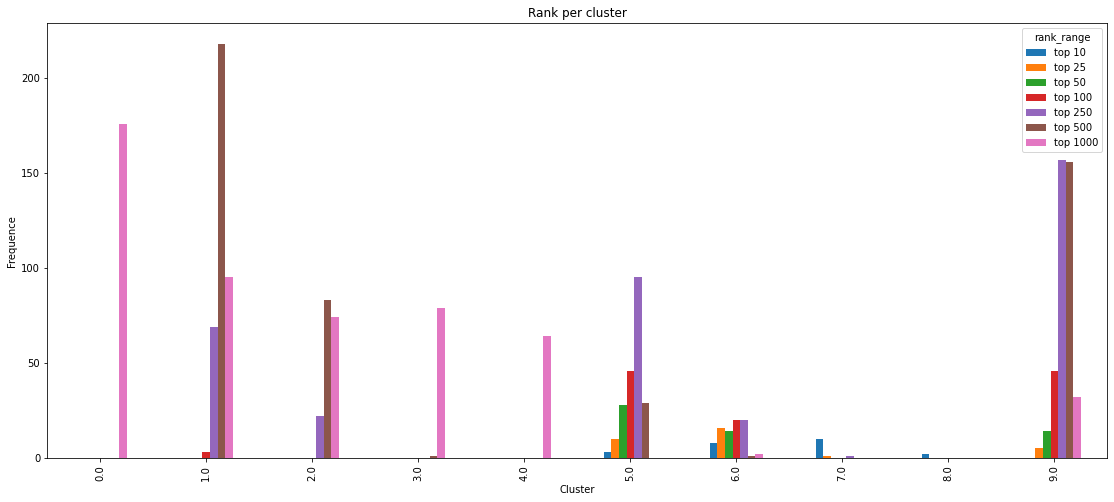
\includegraphics[width=0.62\linewidth]{images/clustering/OtherClusterings/x_means_ranks.png}}
    \caption{X-Means: pca and analysis.}
    \label{fig:x_means}
\end{figure}

By looking at \autoref{fig:x_means} we can see that X-Means separated better the players by their skills than our previous attempts, so we think that it did the best job among everything we tried.

\subsubsection{SOM Soft-Clustering}
From the pyclustering package documentation: this algorithm uses an amount of clusters that should be allocated as the size of a SOM map. The captured objects by the neurons are clusters. We expected the pyclustering library to provide us a way to plot the SOM lattice but this wasn't the case, so we went, as always, with the pca just like the other approaches. For the choice of k we did the same work as K-Means and we found that the best choice was for $k=3$ but we couldn't calculate in any way the SSE since the implementation by the library doesn't come with a way to obtain the cluster centroids, so we only considered the Silhoutte and Davies-Bouldin scores.

\begin{figure}[H]
    \centering
    \subfloat[Clusters generated by SOMsc]{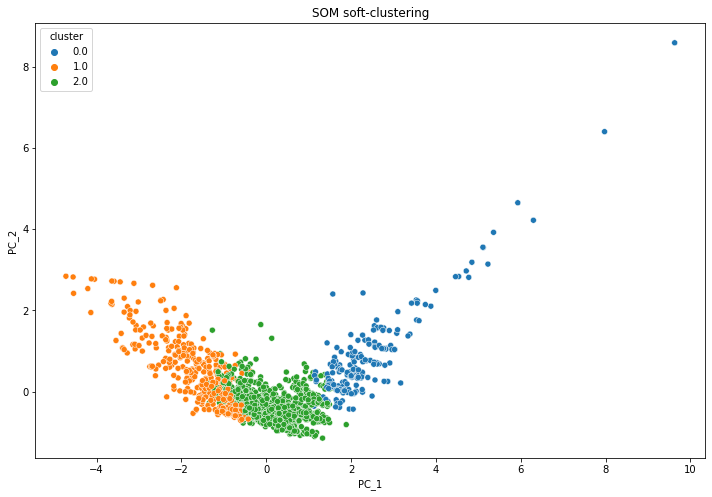
\includegraphics[width=0.48\linewidth]{images/clustering/OtherClusterings/somsc_pca.png}}
    \subfloat[Distribution of players' ranks per cluster]{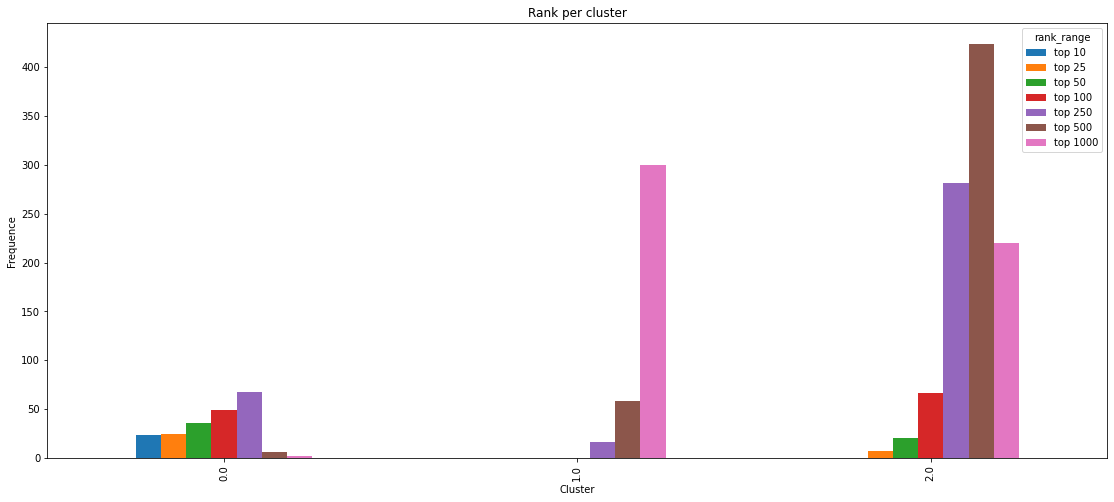
\includegraphics[width=0.52\linewidth]{images/clustering/OtherClusterings/somsc_ranks.png}}
    \caption{SOM soft-clusering: plot along PCAs and analysis.}
    \label{fig:somsc}
\end{figure}

The results obtained, which can be seen on \autoref{fig:somsc}, are similar to the ones obtained by k-means, so we think we don't need to explain anything more about this approach.